\documentclass[red]{beamer}
\mode<presentation>

\usepackage{graphicx}
\usetheme{Warsaw}
\useoutertheme[subsection=false]{smoothbars}

\title{Accelerated Astronomical Source Finding} 

\author{Yaseen Hamdulay and Jarred de Beer}
\institute{{\tiny supervised by} Michelle Kuttel and Sarah Blythe}
\date{26 May 2015}

\begin{document}
\frame{
    \titlepage
}

\section[Outline]{}
\frame{\tableofcontents}

\section{Introduction}
\subsection{Source Finding}
\frame{\frametitle{What is Radio Astronomy Source Finding?}
\begin{itemize}
\item Process of identifying galaxies or other objects from blind surveys
of the sky. 
\item It is made difficult by the amount of noise that gets detected.
\item Traditionally done by astronomers by hand. It's very tedious work.
\item It is estimated that there are one hundred billion galaxies in the universe.
It will be impossible for any team of humans to catalogue this. 
\end{itemize}
}

\frame{\frametitle{Survey Example: Noisy}
\centering 
\includegraphics[scale=.75]{noisenoisegalaxy}
}

\frame{\frametitle{Survey Example: Denoised}
\centering 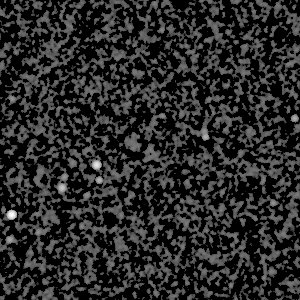
\includegraphics[scale=.75]{noisenoisenoisegalaxy}
}

\frame{\frametitle{Automated Methods}
\begin{itemize}
%It is clear that we need automated methods of source finding.
\item There exist automated source finders with DUCHAMP being the
most well known. 

\item With the next generation of Radio Interferometers we are
expecting current generation source finders to take between
hours and days.

\item We are proposing using GPU's to accelerate the source finding process.
\end{itemize}
}

\subsection{GPU}
\frame{\frametitle{GPU}
\begin{itemize}
\item GPU's are low-cost highly parallel coprocessors. 
\item Difficult to program on due to highly parallel nature and unusual memory hierarchy
\end{itemize}
}

\section{Work Distribution}
\frame{\frametitle{Work Distribution}
\begin{itemize}
\item We intend to work on two source finders independently. This prevents either of us from blocking the other.
\item Source finders perform differently with respect to completeness and reliability as they often trade one off for the other.
\item \textbf{Reliability} is the ratio of true positive detected sources to total sources.
\item \textbf{Completeness} is the ratio of sources detected to actual sources.
\item It is useful to have a variety of source finders depending on an astronomers work load. 
\end{itemize}
}

\section{Source Finders}
\subsection{Yaseen (DUCHAMP)}
\frame{\frametitle{Yaseen, DUCHAMP}
\begin{itemize}
\item DUCHAMP is a complete source finding package that is well-known in the astronomy community
\item According to Popping et al DUCHAMP performs the best in terms of completeness and reliability
for point sources and one of the best for larger galaxies which makes it a good target for acceleration. 
\end{itemize}
}

\frame{\frametitle{Pipeline overview}
\begin{figure}
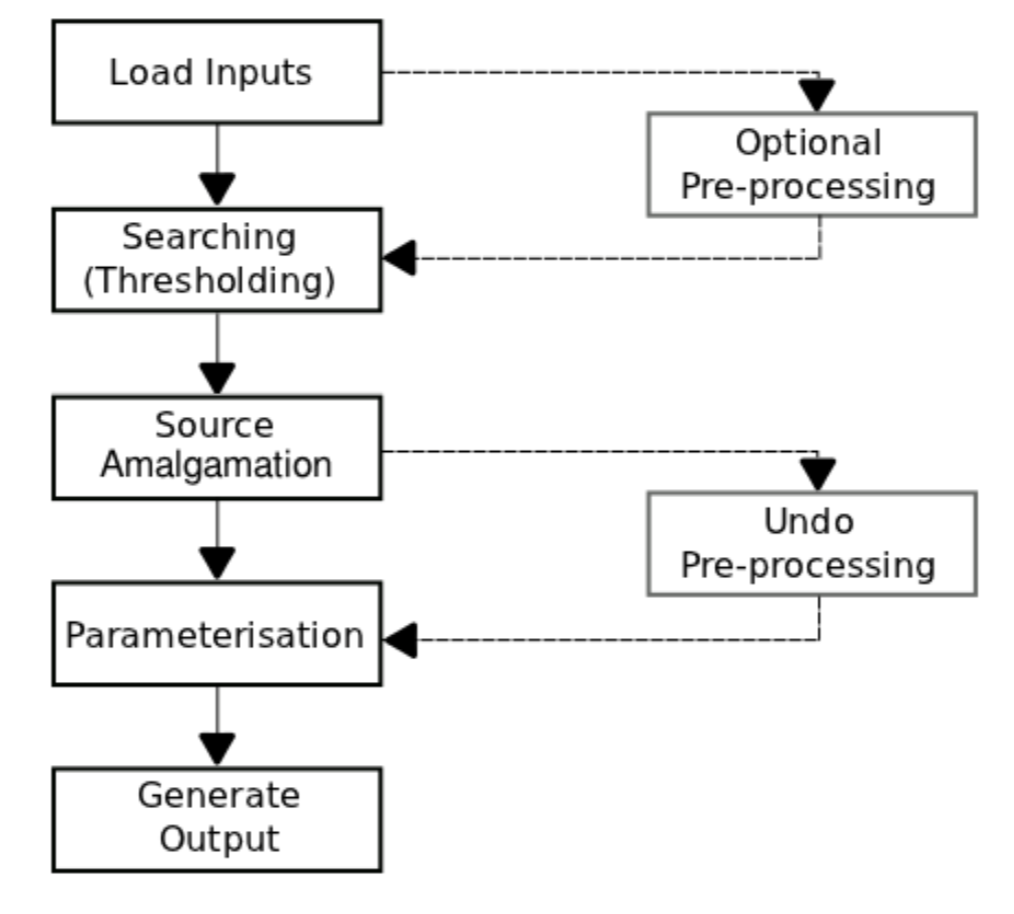
\includegraphics[scale=.3]{duchamp-pipeline}
\caption{DUCHAMP pipeline}
\end{figure}
The DUCHAMP package takes a data cube and pushes it through a pipeline
with data cube at one end and the parameterised sources at the other.

% wavelet reconstruction up to 92% of run time
% a'trous wavelet reconstruction is essential to DUCHAMP's performance
}

\subsection{Jarred (SoFia, Smooth and Clip Filter)}
\frame{\frametitle{Jarred, SoFia: Smooth and Clip filter}
}


\section{Related Work}
\frame{\frametitle{Related Work}
\begin{itemize}
\item Selavy, CPU parallel implementation of DUCHAMP.
\item Badenhorst et al also did a CPU parallel implementation of the wavelet reconstruction filtering algorithm.
\item Parallel Gaussian Source Finder has been ported to the GPU with massive performance improvements.

\end{itemize}
}

\section{Testing}
\frame{\frametitle{Testing}
\begin{itemize}
\item The primary goal of this project is to accelerate the source finding
process. Our most important metric is therefore execution speed.
\item The execution time of the overall source finder depends on the data
cube it is executing on. We should keep this constant or use predetermined
data cubes.
\item Compare against single threaded implementation.
\item Ensuring correctness is of utmost importance.
\end{itemize}
}

\end{document}
